\cleardoublepage
\chapter{Outputting Content for Deployment and Performance}
\label{ch:10}

%------------------------------------------------

\section{Perform Mode}

\begin{fullwidth}
Perform mode should be used whenever possible when deploying projects. The basic premise behind Perform mode is that when a project is ready to be delivered, it will be in a state that won't require on-demand programming, and thus won't require the Network editor. It is surprising how much system resources can go towards just rendering the Network editor, especially if there are many Operators with visible viewers, displaying CHOP channels, TOP previews, DAT tables, etc.

Therefore, Perform mode exists so that that computer can focus on rendering the content, and doesn't have to render the extra Network editor. Everything that is involved with creating the final product is still rendered and active in Perform window, including elements such as external data inputs and outputs. The only thing that stops being rendered is the Network editor.

As mentioned in the Component chapter, it is recommended that Container COMPs are used as the source for Window COMPs. The same recommendation applies to Perform mode.

Open example 'Perform\_mode.toe'. In this example, the Container COMP, 'container1', is used as the source for Perform mode. Press the 'F1' key to enter Perform mode, and the contents of the container will be displayed in a new window. Press the 'ESC' key to exit Perform mode and return to the Network editor. There is a UI button that can be used to enter Perform mode via the mouse.

\begin{center}
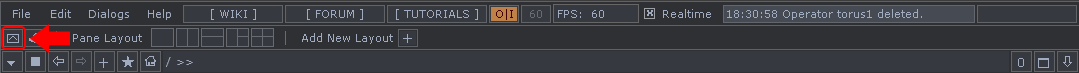
\includegraphics{./img/10.1/perform.png}
\end{center}

\end{fullwidth}

%------------------------------------------------

\section{Performing with the Network Editor}

\begin{fullwidth}

Every situation is different, and it is possible that programming might have to be done during a live performance. If that is the case, there are a few things that can help manage the impact the Network Editor has on the system. The first is to turn off the viewers on any Operators that don't need to be monitored. See the diagrams below:

\begin{center}
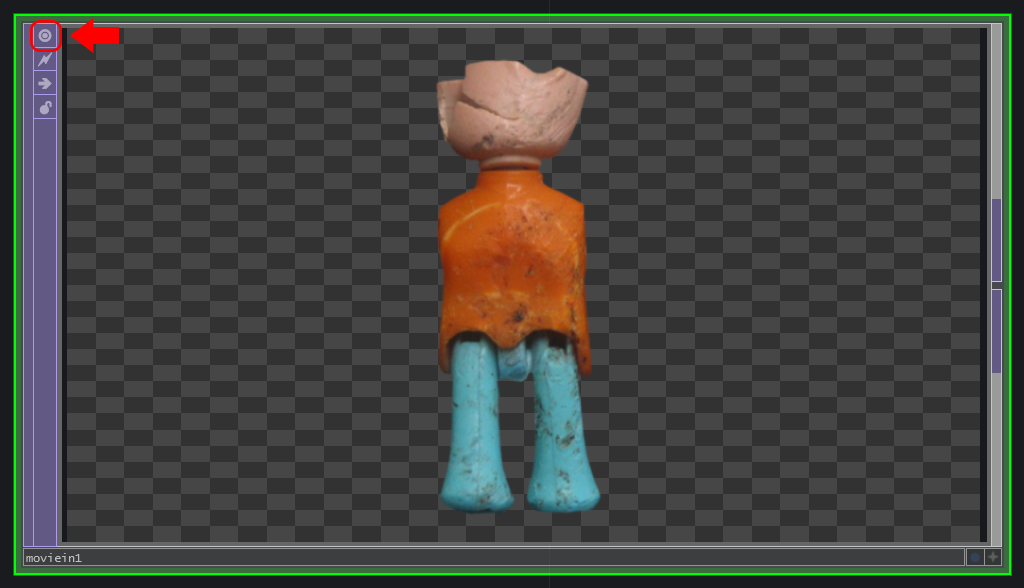
\includegraphics[width=12cm]{./img/10.2/performing-network-1.png}

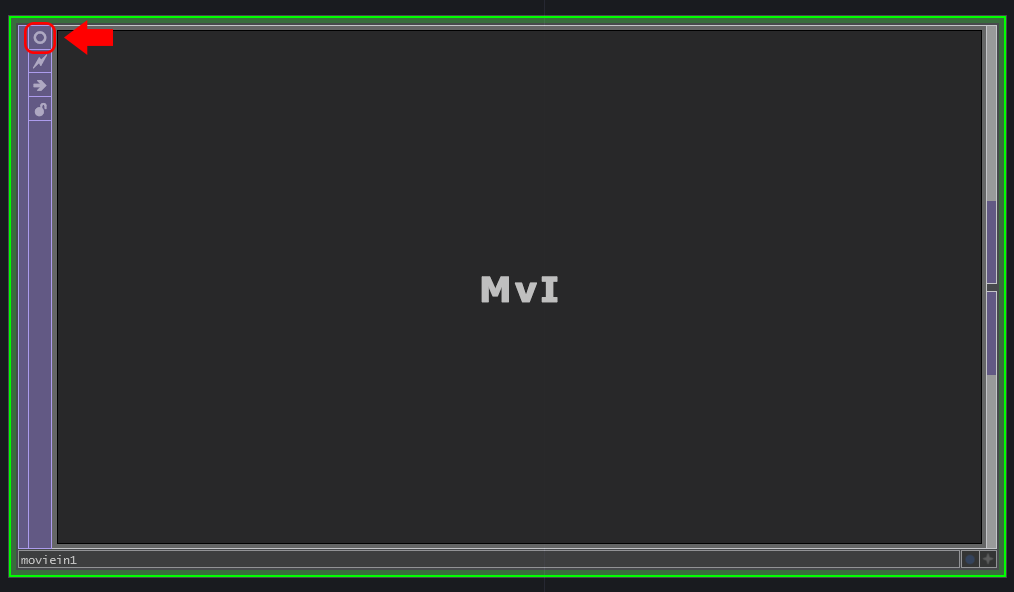
\includegraphics[width=12cm]{./img/10.2/performing-network-2.png}
\end{center}

The next thing that helps is to only use 1 pane in the Network Editor. The more panes that are visible, the more things there are needing to be rendered. 

Finally, moving in and out of large Networks should be avoided. Moving in and out of large Networks can cause frame drops, as TouchDesigner will have to render all of the Operators in that Network before they can be viewed. 

\end{fullwidth}

%------------------------------------------------

\section{Creating an Output Raster}

\begin{fullwidth}

As a general rule, to get the best performance possible, one should always strive to only use 1 Window COMP at a time. This doesn't apply while programming, but when it comes to deployment and performance, having more than one window open will greatly decrease the systems performance. So what should be done if there are multiple outputs with different positions and rotations?

The answer is to create a raster for the output and create a single, all-encompassing, window that will span all of the real-world outputs.

This is more simply expressed with an example. In this example scenario, there are four SXGA+ projectors, each with a resolution of 1400x1050. In the real-world setup, there are two projects beaming horizontally on side walls, and two projectors beaming vertically, and edge blended, on the center wall. The diagram below illustrates the desired setup.

\begin{center}
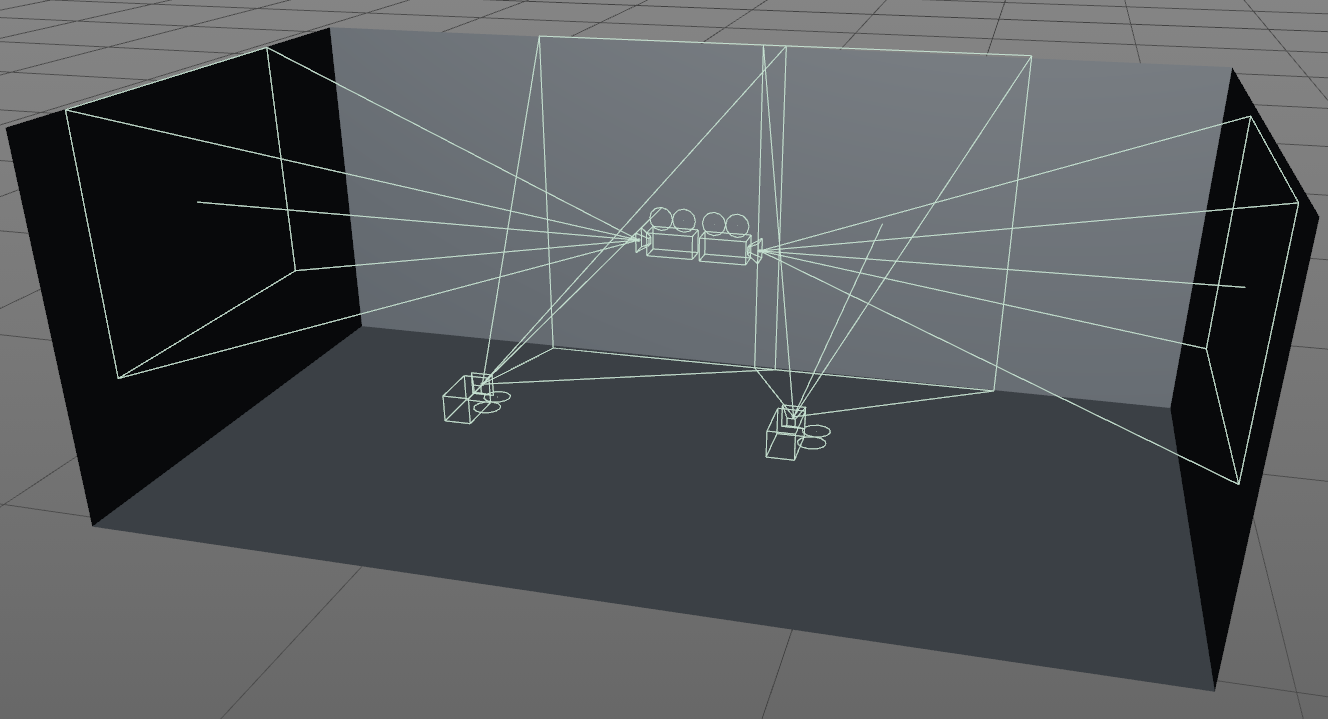
\includegraphics{./img/10.3/raster-1.png}
\end{center}

This setup isn't particularly complex, thus knowing how to deal with it most effectively is important. Let's take this setup, and lay it out in 2D. 

\begin{center}
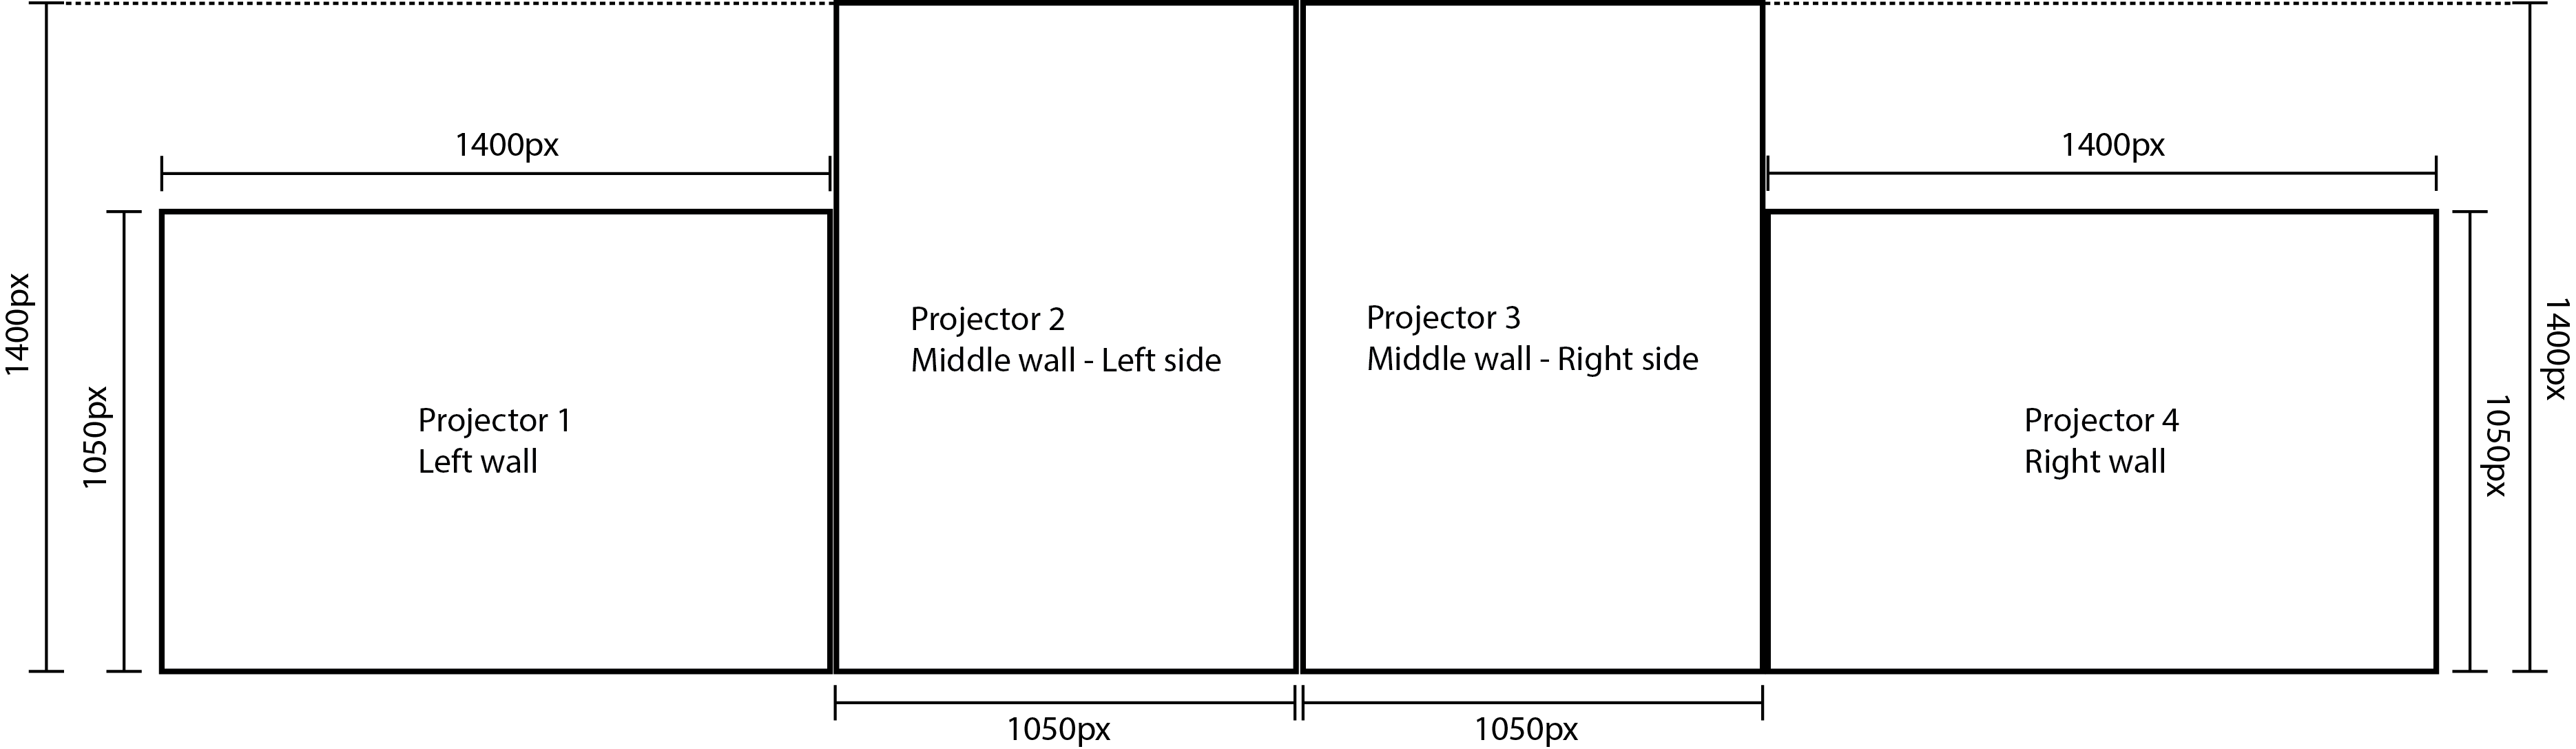
\includegraphics{./img/10.3/raster-2.png}
\end{center}

A beginners's first instinct might be to use four Window COMPs because there are four outputs, two of which need to be rotated. The challenge is finding the most efficient layout for these four canvases, to create a single raster. In this instance, because all four outputs are the same resolution, an easy solution is to make a 2x2 grid. 

\begin{center}
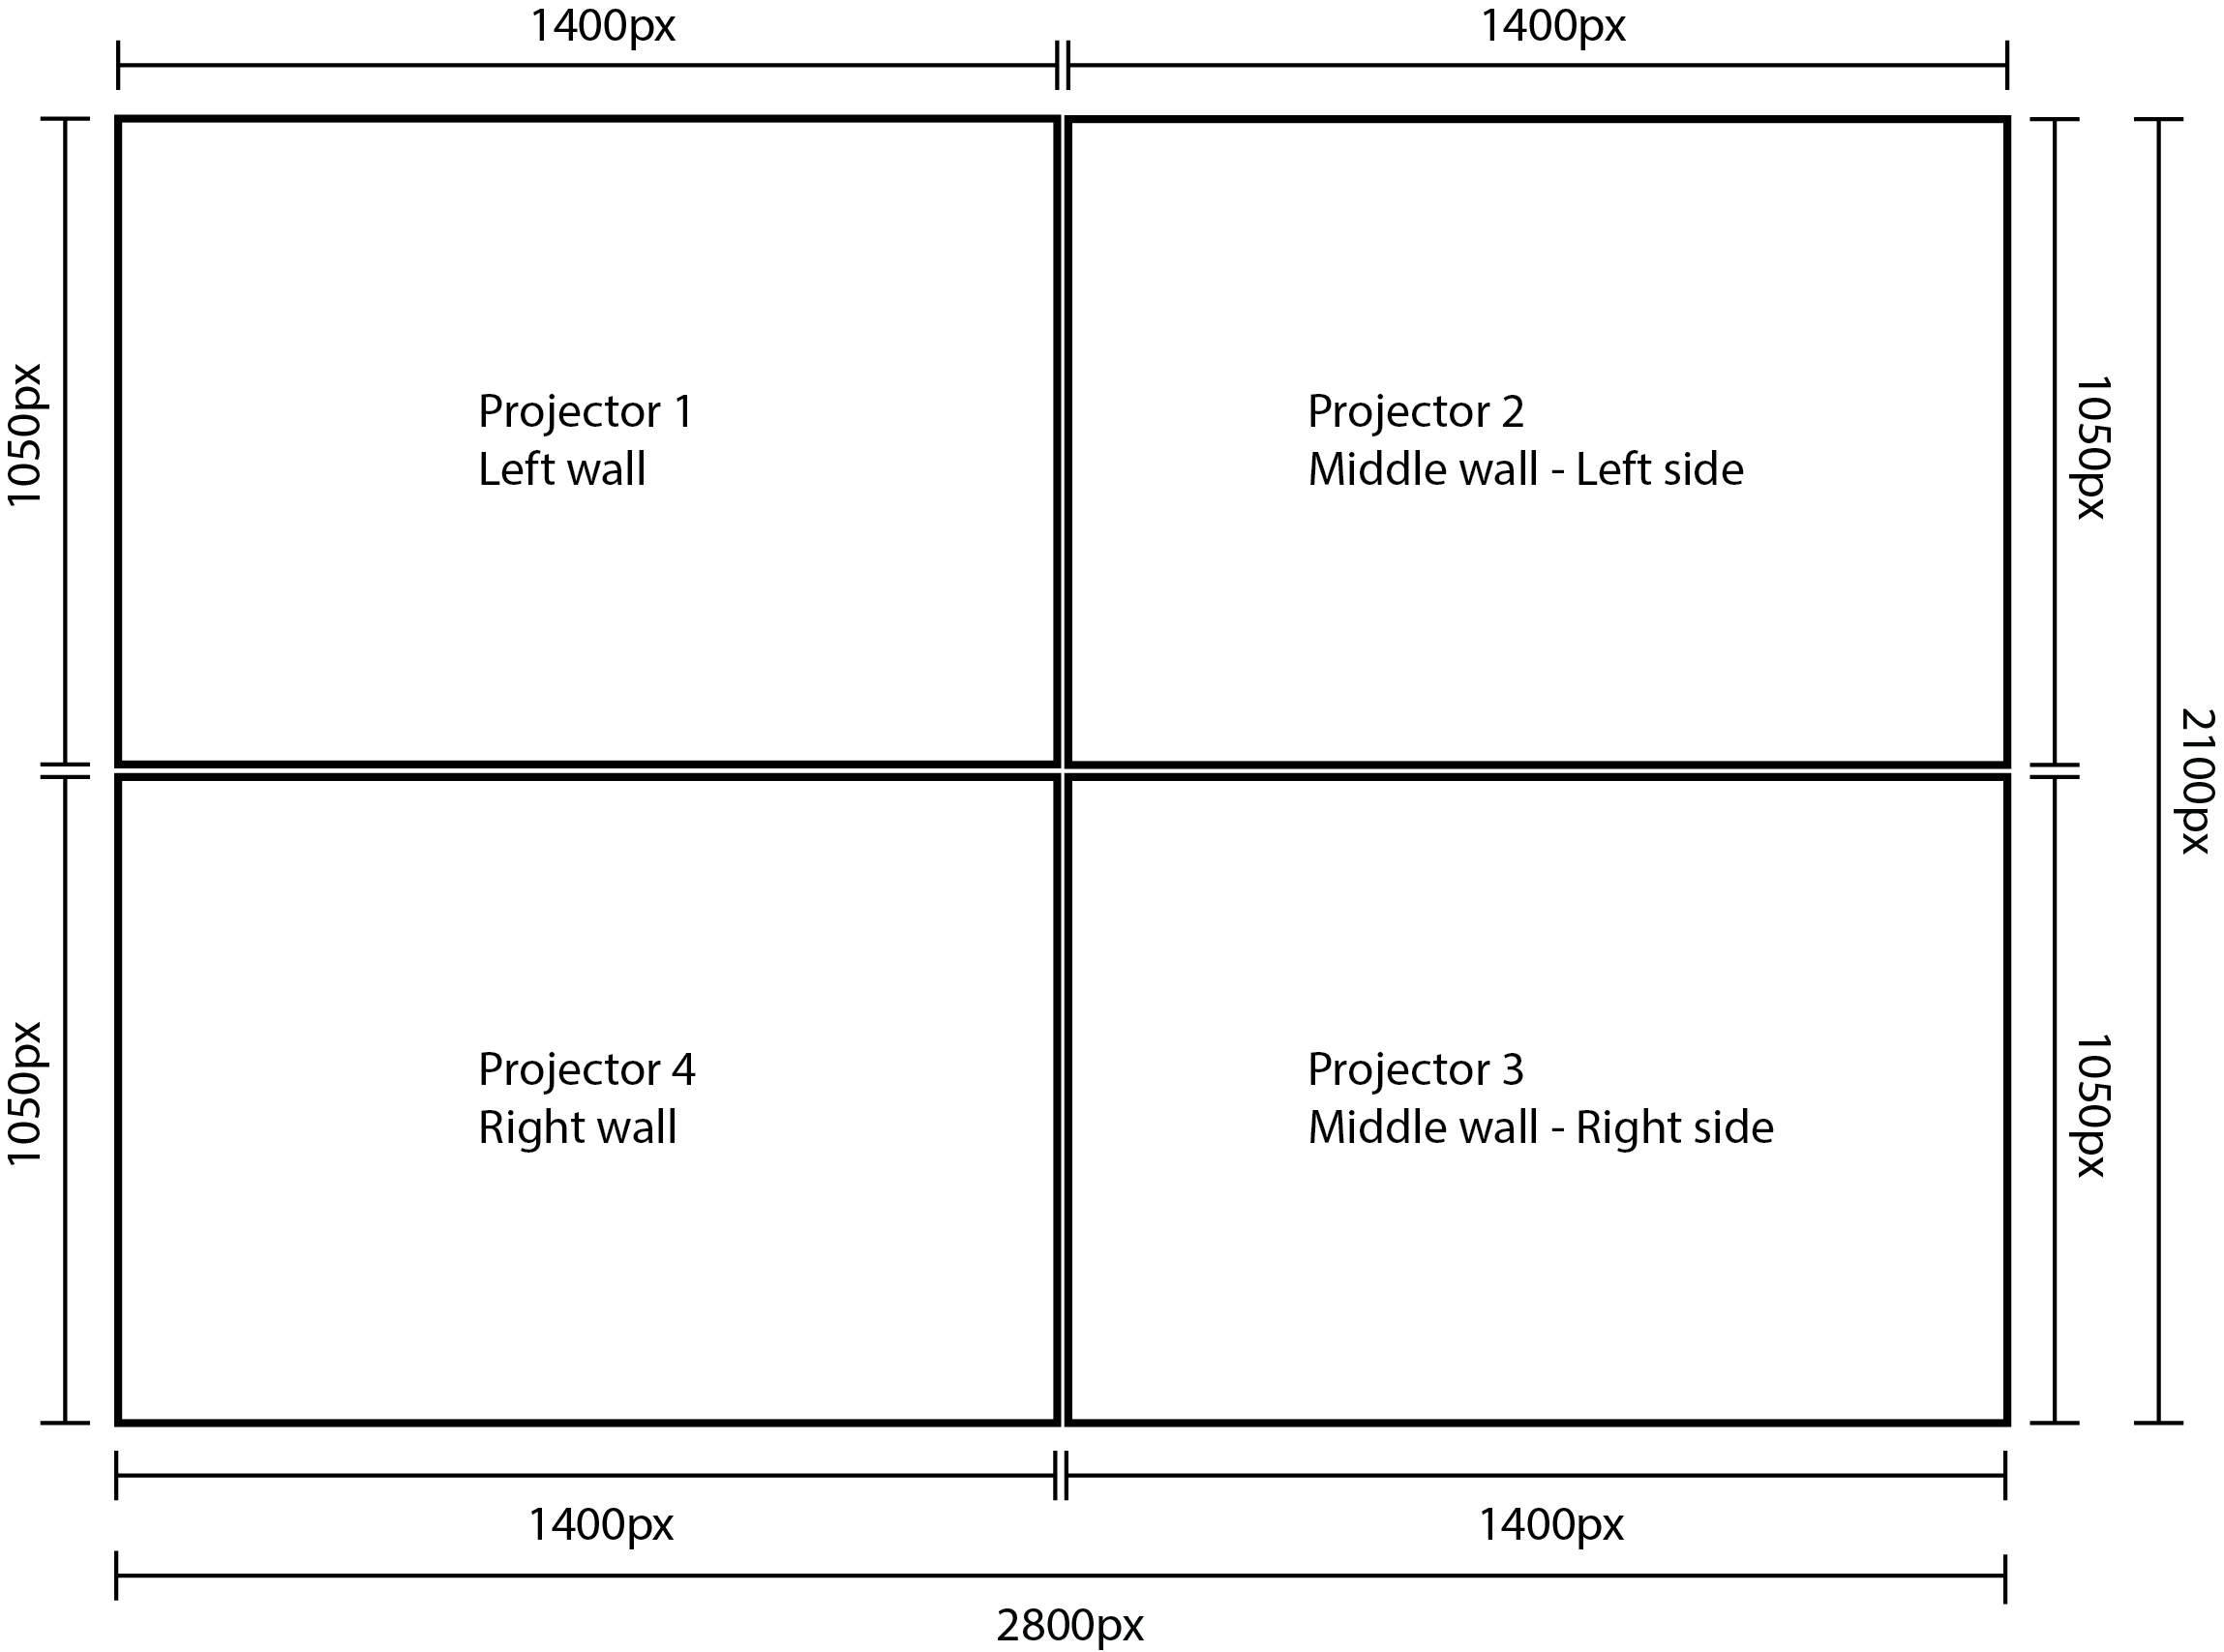
\includegraphics{./img/10.3/raster-3.png}
\end{center}

In the above diagram, all of the outputs are placed into a single raster. This setup can efficiently use one Window COMP that is 2800x2100 pixels. At this point, the nVidia or AMD control panel should be used to create a similar setup out of the monitors in Windows, which should then be connected to the correct outputs on the graphics card.

The next step is to prepare this raster inside of TouchDesigner. Open example 'Raster.toe'. There are a few things to note from the start. For the example, some very basic dummy content has been created, and will represent where real content would go. 'Content1' is for the left wall projector and is 1400x1050 pixels. 'Content2' is for the middle set of projectors and is 2100x1400 pixels. 'Content3' is for the right wall projector and is 1400x1050 pixels. All of the canvas building happens inside of the 'canvas' Container COMP.

In the 'canvas' container, the signal path can be followed from left to right, and from top to bottom, like a waterfall. The first step is to create a blank raster that content can be composited on. There is a Constant TOP set to 2800x2100 pixels at the top left of the Network for this purpose. Using an Over TOP, the first piece of content is placed, for the left wall projector, in its appropriate position, according to the diagram above. This is done using the 'Translate' parameter of the Over TOP. Projector 1: done!

The middle wall has two projectors that are edge blended together. Because a few operations need to happen on the raw content, there is a container name 'crop'. This keeps the operations encapsulated, neat, and easy to find. Inside of 'crop', three main operations are performed. The first is that the big piece of content is cut it in half, so that each projector can display half of the image. Since the projectors are positioned vertically in the installation, but are positioned horizontally in the raster, the 'Flop' parameter of the Flip TOP is used to turn the canvas on its side. The settings for the Flip TOP will always end up being different depending on hardware setup, so be prepared to try different Flip and Flop settings to get the correct content orientation.

Side note: Most beginners have trouble rotating a full canvas. The first instinct is to use the Transform TOP, but it is important to note that the Transform TOP will transform the pixels inside of a canvas. This is where the 'Flop' parameter of the Flip TOP comes in. It will fully rotate the canvas.

Since this example isn't dedicated to edge blending, the 'edge\_blend' containers are just place holders that create the visual effect of a blended edge. 

With all the cropping, rotating, and blending done, the two projector outputs are ready to be composited onto the raster. Using the same technique as before, an Over TOP with a modified 'Translate' parameter correctly positions the two pieces of content. Now Projector 2 and 3 done as well!

The final projector is as simple as the first, and using the trusty Over TOP, the final piece of the puzzle is positioned.
 
As mentioned in an earlier chapter, it is best practice to use Container COMPs instead of TOPs as the source for Window COMPs. In this project, there is a container that is 2800x2100 pixels that holds the completed raster. The 'final' container is set as the Window COMPs 'Operator', the 'Borders' setting is turned off in the Window COMP, and the window size is set to 2800x2100 pixels. With that, the project is ready to be output to the above, 4 projector, setup.

\end{fullwidth}

%------------------------------------------------

\section{Displays, Tearing, and Stuttering}

\begin{fullwidth}

There has not been much hardware discussion throughout this book, but it is important to keep a few things in mind when working with multiple displays. The most important rule is to always try to have all display hardware be exactly the same. Any difference in the signal flow, can cause what is called 'tearing'. The image below is an example of a frame that has tearing.

Examine the image below. Is it an example of what a frame with tearing will look like. Notice the two horizontal cuts across the frame:

\vspace{10mm}

\begin{center}
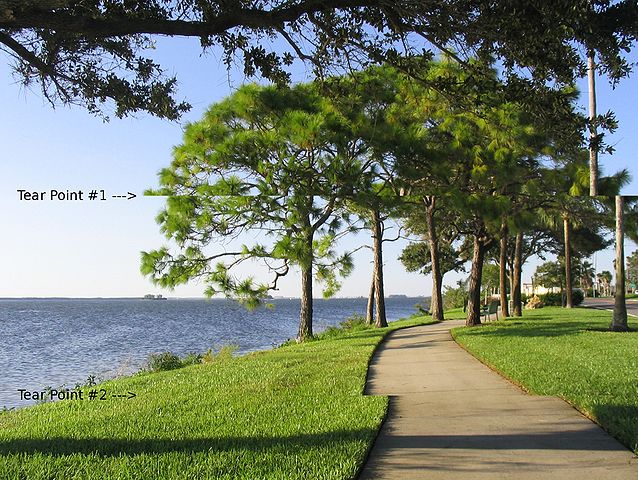
\includegraphics{./img/10.4/tearing.jpg}
\begin{footnotesize}
Image courtesy of Wikipedia
\end{footnotesize}
\end{center}

Tearing occurs when a display refreshes its image out of sync with when the graphics card renders its image. The result is part of the image being from the previous frame, and part of it being from the next frame. On slow moving content, this can sometimes be hard to notice, but once there is any sort of motion in the content, tearing becomes incredibly distracting.

Tearing is a complex issue to solve, but there are a few preventative measures that can be taken to avoid it. The first is to use a professional graphics card, such as something from the nVidia Quadro series. Most companies will not guarantee tear-free playback on anything but their professional cards.

The second is to always ensure that the displays are identical. Identical can't be stressed enough. If there is an installation with 3 outputs that have a refresh rate of 60hz, and one output with a refresh rate of 59hz, there is a chance there will be tearing. If there is an installation with two 1080p projectors, and two SXGA+ projectors, there is a chance there will be tearing. The best practice is to use displays that are not only identical in specifications, but are also the exact same model of displays. Network remote access applications like VNC and LogMeIn have also been the culprits of tearing.

This brings up a very important issue with tearing: there are no hard and fast rules. Sometimes, setups with a handful of different resolutions and refresh rates will work perfectly and won't tear. On the other hand, sometimes even setups with identical displays can tear. Enough emphasis cannot be put on preventative measures to avoiding tearing. When tearing issues arise, the only things that can be done are a step by step breakdown and analysis of the system to see what is causing the tearing.

There is a list of common debugging methods on the Derivative Wiki page for 'Tearing'. 

Generally the steps to begin with are as follows, in no particular order:

\begin{itemize}
\item Verify the project isn't dropping any frames. Dropped frames can sometimes trigger tearing
\item Verify no other applications are interrupting or mirroring the graphics card drivers, such as VNC and LogMeIn.
\item Disconnect every display connected to computer, and one by one connect them until tearing occurs. Then isolate that display on it's own, and figure out if it's being cause by a single display, or by the layout
\item Verify all displays are configured to the same resolution, colour bit depth, and refresh rate, in the nVidia or AMD control panel
\item Verify that none of the displays have any rotation applied in Windows. this can cause unpredictable behaviour.
\item Check the graphics card driver version and update it if necessary
\item Check for drivers or firmware updates on external video splitters - such as the Datapath X4 or Matrox TripleHead2Go
\item Confirm only 1 Window COMP is being rendered
\item Verify Windows Aero is disabled. In Windows 7, Aero can cause dropped frames and stutters, but won't tear. Once disabled, the system might tear, but stutter free playback is guaranteed.
\item Configure a Premium Mosaic using the nVidia Control Panel to create a single logical display 
\end{itemize}

There are many instances in which a system that performs perfectly, and doesn't drop a single frame, will occasionally stutter. This may occur because of how displays and graphics cards negotiate different refresh rates. 

If a project is running at 30 FPS, but a display's refresh rate is 60hz, frame doubling has to be negotiated somewhere. Between the graphics card and the display, most of the time this negotiation is done transparently, but sometimes there can be issues. What can occur is that instead of negotiating a proper frame doubling for every frame, one frame might be displayed once, while the next frame is displayed for three frames. From the project's point of view, no time is lost and no frames were dropped, so it would not be reported in the Performance Monitor or Windows Task Manager. 

If it seems that this kind of issue may be occurring, use the 'FPS is Half Monitor Refresh' feature in the Window COMP. This informs the graphics driver that it should show each frame for 2 refreshes.


\end{fullwidth}
